\subsection{Methodology}
\subsection{Data Collection}
\label{subsec:datacollection}

We deployed a data collection system to look for more realistic information about lifetime and bandwidth consumption through time of Tor circuits. Our objective is to have a deeper understanding of typical Tor usage, and if such usage can benefit from our channel-based payment system. For example, those measurements could capture some notion about the type and magnitude of potential premium traffic. We define the type of traffic based on the port used to connect to the request service. Besides the classical ports 80 and 443 for web traffic, we aggregate data based on some other families, such as the WHOIS protocol~\cite{rfc3912} and RWHOIS~\cite{rfc2167} with port 43 and 4321. The complete list of families is constructed from the reduced exit policies~\cite{reducedexitpolicies} we run on our relays. It allows us to reason based on application specific traffic.
%We interested to know about the distribution lifetime of Tor circuits for each port we allow. We are also interested to picture how many cells those circuits handled through their lifetime with some level of granularity.

\subsubsection{Efforts to preserve users privacy}

\subsubsection{Observations}

\begin{figure*}
	\centering
	\begin{subfigure}[t]{0.32\textwidth}
		\centering
		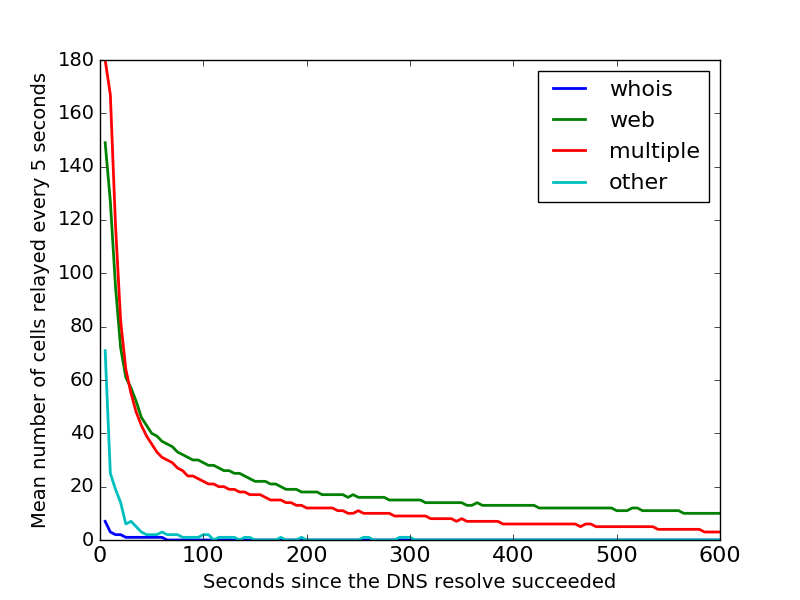
\includegraphics[scale=0.28]{images/exitmeasurement.png}
		\label{fig:stats_a}
	\end{subfigure}
	\begin{subfigure}[t]{0.32\textwidth}
		\centering
		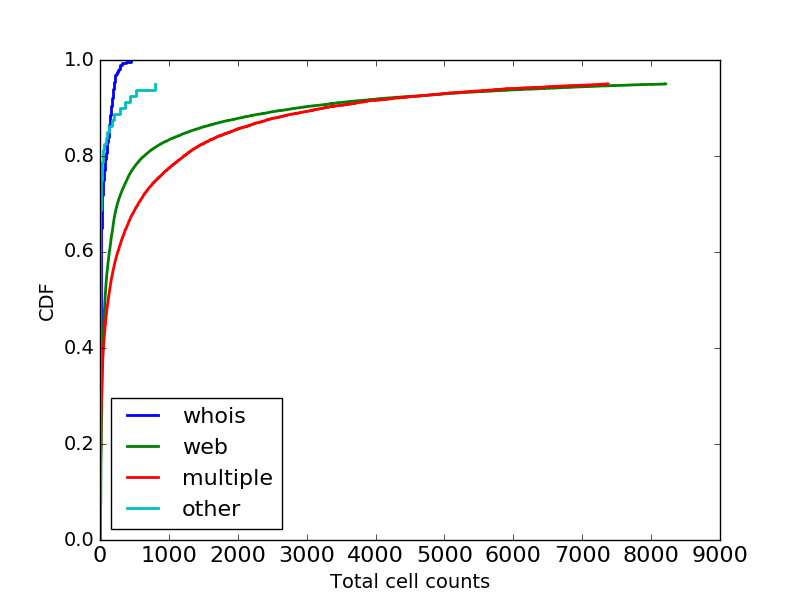
\includegraphics[scale=0.28]{images/totcellcountscdf.png}
		\label{fig:stats_b}
	\end{subfigure}
	\begin{subfigure}[t]{0.32\textwidth}
		\centering
		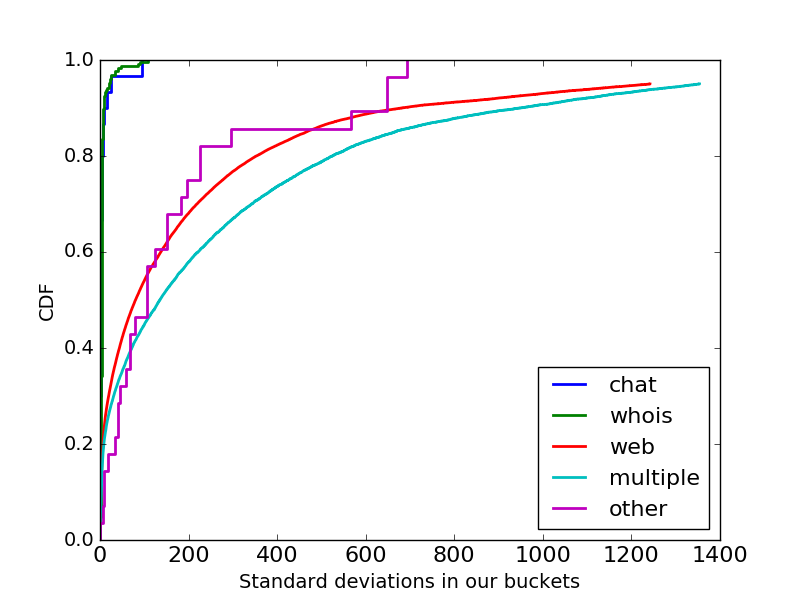
\includegraphics[scale=0.28]{images/stddevs.png}
		\label{fig:stats_c}
	\end{subfigure}
	\label{fig:measurements}
	\caption{Tor measurements}
\end{figure*}
\subsection{Ethical Considerations}
